\documentclass{ceel}

% ===========================
%Coloque aqui pacotes adicionais, se necessário
\usepackage{hyperref}
\usepackage{verbatim}
\usepackage{array}
\usepackage{amsmath}
\usepackage{subcaption, float}
%%===========================

% Dados do trabalho
\title{Fundamentos Físico-químicos e Matemáticos de um Memristor}

\author[1]{\underline{Lesly Viviane Montúfar Berrios}\thanks{leslymontufar@ufu.br}}
\author[1]{Cibelly Cristina Rodrigues Couto\thanks{cibelly.cris@ufu.br}}
\author[1]{Yasmin Delbany Cury\thanks{yasmin.cury@ufu.br}}
\author[2]{Paulo Henrique Oliveira Rezende\thanks{paulohenrique.rezende@ufu.br}}

\affil[1]{FEELT - Universidade Federal de Uberlândia}
\affil[2]{FEELT - Professor Adjunto - Universidade Federal de Uberlândia}

\begin{document}

\inserirtitulo

\begin{multicols}{2}

\textbf{\emph{Resumo} - Um estudo sobre o comportamento do quarto elemento de circuito fundamental idealizado por Leon Chua em 1971 e implementado primeiramente pela equipe da \emph{HP Labs} liderada por R. Stanley Williams em 2008 é apresentado. Chamado de \emph{memristor}, o novo elemento de circuito passivo de duplo terminal relaciona as variáveis de carga $q(t)=\int_{-\infty}^t i(\tau)\, d\tau$ e fluxo $\varphi(t)=\int_{-\infty}^t v(\tau)\, d\tau$ e comporta-se como um resistor não-linear com memória. Sua propriedade peculiar advém da capacidade do material de manter seu último estado, e permite aplicações em diversos contextos, como em memórias ReRam e inteligência artificial.} %% aplicacoes a completar
\vspace*{10pt}

\textbf{\emph{Palavras-Chave} - Inteligência Artificial, Memórias ReRam, Memristor.}


\begin{center}

%Insira aqui o Título do trabalho em inglês
\noindent\textbf{\large \uppercase{Physicochemical and Mathematical Foundations of a Memristor}}
\end{center}

\textbf{\emph{Abstract} - A study of the behavior of the fourth fundamental circuit element devised by Leon Chua in 1971 and first implemented by the \emph{HP Labs} team led by R. Stanley Williams in 2008 is presented. Called \emph {memristor}, the new two-terminal passive circuit element lists the variables of charge $q(t)=\int_{-\infty}^t i(\tau)\, d\tau$ and flux $\varphi(t)=\int_{-\infty}^t v(\tau)\, d\tau$ and behaves like a nonlinear resistor with memory. Its peculiar property comes from the material's ability to maintain its last state, and allows applications in various contexts, such as ReRam memories and artificial intelligence.}
\vspace*{10pt}

\textbf{\emph{Keywords} - Artificial Intelligence, Memristor, ReRam memories.}


\section{Introdução}
%% completar com a palestra de R. Stanley Williams
A teoria de circuitos elétricos, há 150 anos, abrangia basicamente três componentes passivos fundamentais: o capacitor (1745), o resistor (1827) e o indutor (1831). No entanto, em 1971, o professor phD da Universidade da Califórnia, Leon Chua, apresentou novas considerações a partir da análise das possíveis combinações entre as quatro variáveis fundamentais de circuitos: corrente elétrica $i$, tensão elétrica $v$, carga elétrica $q$ e fluxo magnético $\varphi$ – sendo as duas últimas descritas como integrais no tempo da corrente, $q(t)=\int_{-\infty}^t i(\tau)\, d\tau$, e da tensão, $\varphi(t)=\int_{-\infty}^t v(\tau)\, d\tau$, respectivamente.

Chua observou que o capacitor é definido pela relação entre carga $q(t)$ e tensão $v(t)$ via $qd=C dv$. Similarmente, o resistor pela relação entre corrente $i(t)$ e tensão $v(t)$ via $dv=R di$, e o indutor pela relação entre fluxo magnético $\varphi(t)$ e corrente $i(t)$ via $d\varphi(t)=L di$. Teria-se então que a combinação das quatro variáveis fundamentais de circuitos resultaria em somente três componentes fundamentais.
% passivos.
Desse modo, baseando-se no argumento da simetria, o estudioso postulou que haveria um elemento de circuito faltante, capaz de associar a carga $q(t)$ e o fluxo magnético $\varphi(t)$, o que o levou, em 1971, a publicar um artigo no qual idealiza o novo componente, definido pela relação $d\varphi=M dq$ e que denominou \emph{memristor}, uma contração de \emph{memory resistor} \cite{artigo}. 

%, em português \emph{resistor com memória} 
Portanto, considerado como o quarto elemento fundamental dos circuitos eletrônicos, ao lado do capacitor, resistor e indutor, o \emph{memristor} destaca-se por apresentar uma propriedade peculiar, cuja explanação e abordagem teórica é tratada adiante. É definido, assim como um resistor, como um componente eletrônico passivo de duplo terminal, utilizado para limitar a corrente em um circuito e dissipar energia térmica, com o diferencial de que, para o \emph{memristor}, essa limitação, chamada de resistência ou impedância, alterar-se conforme a quantidade de carga elétrica que flui em si e mantém o valor da última resistência obtida até a aplicação de nova carga.

Apesar da proposta teórica do \emph{memristor} ter sido apresentada por Chua em 1971, sua primeira implementação prática ocorreu apenas em 2008, nos \emph{Laboratórios da Hewllet-Packard} (\emph{HP}), graças à equipe liderada pelo físico-químico Dr. Richard Stanley Williams, que desenvolveu linhas de memristores com base no dióxido de titânio ($TiO_2$) em escala nanométrica \cite{nature}. A demora deve-se, principalmente, à dificuldade em encontrar materiais que fossem capazes de conferir a propriedade de reter memória ao dispositivo eletrônico e que satisfizessem a base teórica apresentada por Chua \cite{artigo}.
Dessa forma, o componente recentemente sintetizado contém a propriedade da não-volatilidade, que, aliada a possibilidade de ser trabalhado em escala nanométrica, o torna promissor em aplicações e garante sua contribuição na validação da Lei de Moore.

Pissardini \cite{memcomputacao} atenta para aplicações de \emph{memelementos} na elaboração de novas arquiteturas computacionais, que, corroborado pelos ideais da Arquitetura de Von Neumann, são capazes de realizar tarefas específicas. Essa abordagem tem sido conhecida como \emph{memcomputação}.
%% que tarefas? não sei

%% completar paragrafo de aplicacoes:
%% circuitos lógicos CMOS
%% voice encryption - drive
%% memória ReRam !!
%% Computacao neuromorfica, AI, redes neurais CNN
%% Termistores - proposto primeiramente por Chua

Sob essa perspectiva, a temática deste artigo basear-se-á na descrição detalhada desse novo componente, nos âmbito físico, químico, eletrônico e matemático, com intuito de compreender como o mecanismo interno converge para as propriedades impostas,  por Chua, a um dispositivo \emph{memristor}. É de interesse ainda discutir acerca das aplicabilidades do dispositivo, para assim poder expor o impacto de sua descoberta na teoria de circuitos e importância para o crescimento tecnológico. %% eletronico com SPICE
%% se formos acrescentar mais alguma coisa como circuito LTSpice.
%% depende das aplicacoes

Na Seção \ref{estrutura} são apresentadas as características estruturais, físico-químicas, de um \emph{memristor}, com ênfase para o modelo da \emph{HP Labs}. Para, na Seção \ref{analise-matematica}, analisá-lo matematicamente e, assim, provar a natureza de suas propriedades e peculiaridades a partir do equaciomento e disposição de gráficos. Além disso, a Seção \ref{sim} apresenta simulações computacionais nos ambientes \emph{MATLAB} e \emph{LTSPICE} que exemplificam suas características marcantes. Finalmente, na Seção \ref{aplicacoes}, é explicitada algumas de suas aplicações e recentes estudos.


%% precisa colocar imagem pequena para explicar que a propriedade do memristor deve-se basicamente à redistribuição das lacunas(+) devido à deficiencia em oxigenio.
%% de preferencia a msm imagem do R. Stanley Williams
\section{Características estruturais de um memristor} \label{estrutura}
Dispositivos de resistência variável baseados em óxidos 
possuem vasta aplicabilidade, devido à capacidade de reter memória, pois
admitem características de alta velocidade, alta densidade e operação em baixa energia, 
assim como a não-volatilidade \cite{conceito}. Desse modo, os materiais óxidos são ideiais para a criação de um \emph{memristor}, sendo recentemente utilizados óxidos de titânio e tântalo ($TiO_x$, $TaO_x$)\cite{us}.

\begin{figure}[H]
\centering

\begin{subfigure}{0.49\columnwidth}
\centering
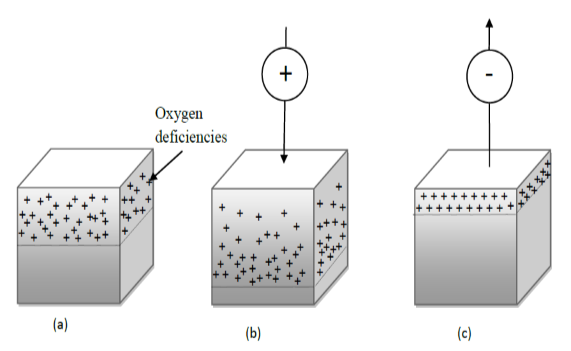
\includegraphics[width=\columnwidth]{oxygen-vacancies}
\caption{Left figure} \label{fig:left}
\end{subfigure}
\hfill
\begin{subfigure}{0.49\columnwidth}
\centering
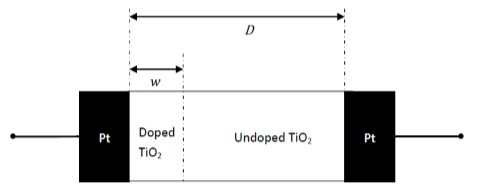
\includegraphics[width=\columnwidth]{HP-model}
\caption{Right figure} \label{fig:right}
\end{subfigure}

\caption{}\label{}
\end{figure}

A fim de cumprir tais características e funções no circuito, o memristor deve ser construído de maneira específica. A estrutura de um dispositivo memristor, basicamente, possui dois eletrodos entre os quais existe uma área isolante, porém com uma nanopartícula que fornece um caminho condutivo entre os eletrodos. %% continuar essa parte
%% aqui comeca assunto diferente, pode ficar para o final da seção
Um memristor pode compreender diversos materiais, sendo os mais utilizados materiais óxidos, geralmente de titânio ou tântalo \cite{us} ($TiO_x$, $TaO_x$).

O funcionamento molecular de um memristor é baseado no movimento de íons livres no meio dielétrico (óxido), o que torna possível o comportamento “memristivo” pois cria mudanças locais na condutividade, causando, assim, a modelagem de filamentos condutores entre os eletrodos. \cite{us}. %% essa é a continuação

Para a formação de tais filamentos condutores entre os eletrodos no meio inicialmente dielétrico (meio entre os dois eletrodos), é necessário realizar um processo conhecido, em inglês, como “electroforming”, ou “eletroformação”. Tal %% o electroforming está na patente?
processo consiste em aplicar uma tensão elétrica suficientemente alta, ou seja, um valor limite, entre os dois eletrodos por um período de tempo suficiente para ser originado um canal condutivo local no meio isolante. O que ocorre é, basicamente, o rompimento da rigidez dielétrica do material que permanece entre os eletrodos. %% explicacao do electrofoming terminou
Os valores limite de tensão e de tempo necessários para ser formado o canal condutivo dependem de qual dielétrico foi utilizado e do material do qual são formados os dois eletrodos, além da estrutura geométrica do dispositivo \cite{us}.Consequentemente, é possível formar diferentes “status” do memristor, como “OFF”, ou seja, um estado de alta resistência; “ON”, ou seja, um estado de baixa resistência, e ainda estados intermediários. %% armazena dados em multinível e não apenas na forma binária. MLC? 
%% Multi Layer Cell ou, traduzindo, Células de Múltiplas Camadas. Esse é o significado de MLC. Aqui, cada célula de memória é capaz de armazenar dois bits em vez de apenas um: 00, 01, 10 ou 11.
%% memórias MLC são muito usadas em SSDs para computadores domésticos.

Para analisar o funcionamento prático de um memristor, pode-se analisar o funcionamento prático de um dispositivo que foi a base para a existência do memristor, o "crossbarlatch", estudado em 2006 pelos %% volta no tempo, poderia colocar essa parte mais para o inicio antes do electroforming
laboratórios da HP. Tal dispositivo passou a ser conhecido como o próprio memristor posteriormente. O "crossbarlatch" era uma espécie de sanduíche, possuindo suas partes externas constituídas por Platina(Pt), com espessura cerca de 3 nanômetros, e sua camada intermediária sendo dividida em duas partes, sendo a primeira formada de óxido de titânio($TiO_2$) e a segunda formada pela mesma substânica, porém deficiente em oxigênio ($TiO_2-x$) \cite{construcao}.  

A parte constituída por $TiO_2$ é conhecida como a parte pura(ou não dopada) e a parte deficiente em oxigênio é conhecida como a parte dopada. Ao se aplicar uma tensão elétrica positiva 
no terminal dopado, as lacunas (onde falta oxigênio) se comportam como cargas positivas e "migram" para o outro lado, ou seja, cargas negativas se deslocam para a parte dopada. Dessa 
forma, a espessura da camada intermediária diminui, ao mesmo tempo que a espessura da camada condutora aumenta, o que resulta na diminuição do valor da resistência do dispositivo. Tal 
estado do memristor é conhecido como "ON", ou baixa resistência. %% Stanley fala isso na palestra, procurar documento que tem oq ele diz na forma de artigo fácil de entender

Por outro lado, ao se aplicar uma tensão negativa no terminal dopado, as lacunas são "atraídas", ou seja, a espessura da camada intermediária aumenta, ao mesmo tempo que a espessura 
da camada condutora diminui, causando um aumento no valor da resistência do memristor. Tal estado é conhecido como "OFF", ou alta resistência. 

Ainda pode-se analisar o comportamento do memristor nos momentos em que não há aplicação de tensão elétrica, ou seja, quando a fonte de alimentação for desligada. Nesta situação, as 
camadas pura e dopada permanecem no mesmo estado que estavam anteriormente. Assim, no momento em que uma tensão for aplicada, a memristência começa do ponto em que tinha 
estacionado antes. %% no momento == quando

Assim, o princípio básico do funcionamento de um memristor é a mudança de posição dos átomos quando sofre influência de uma tensão elétrica, processo que é facilitado por ocorrer em 
escala nanométrica. %% por que? equacao 1/D^2

\section{Fundamentos Matemáticos}\label{analise-matematica}
O \emph{memristor}, a princípio, em 1971, foi definido por Chua \cite{artigo} como elemento de circuito de duplo-terminal caracterizado pela relação do tipo $g(\varphi, q)=0$. Diz-se que 
um memristor é controlado por carga se a relação entre fluxo e carga é expressa como uma função de carga elétrica $q$, e diz-se que é controlado por fluxo se é expressa em função do 
fluxo $\varphi$. Para um memristor controlado por carga tem-se a Equação (\ref{mem-charge}) e derivando-se ambos os termos consegue-se a Equação (\ref{derivate-q}).

\begin{equation}\label{mem-charge}
\varphi = f(q)
\end{equation}

%Derivando ambos os termos da Equação (\ref{mem-charge}):
\begin{equation}\label{derivate-q}
\dfrac{d\varphi}{dt}=\dfrac{f(q)}{dq} \ \dfrac{dq}{dt}
\end{equation}
\vspace{0.1cm}

Sabendo-se ainda que $v(t)=\dfrac{d\varphi}{dt}$ e $i(t)=\dfrac{dq}{dt}$ descrevem, respectivamente, a tensão e corrente elétrica no memristor, 
reescreve-se a Equação (\ref{derivate-q}) como:

\begin{gather}\label{derivate-q}
v(t)=M(q)\ i(t)
\end{gather}

\begin{flalign} \label{M}
\text{onde\qquad} M(q) &=\dfrac{df(q)}{dq}.&
\end{flalign}

$M$ é chamada de \textit{memristência}, e é mensurada na mesma unidade que a resistência (\textit{Ohms} - $\Omega$). A memristência, definida pela Equação (\ref{M}), define uma relação linear entre tensão e corrente, enquanto a carga for constante. Logo se $M$ é constante, o memristor comporta-se como um resistor.

Para um memristor controlado por fluxo tem-se a Equação (\ref{mem-flux}) e derivando-se ambos os termos, a Equação (\ref{derivate-phi}).

\begin{equation}\label{mem-flux}
q = f(\varphi)
\end{equation}

\begin{equation}\label{derivate-phi}
\dfrac{dq}{dt}=\dfrac{f(\varphi)}{d\varphi} \ \dfrac{d\varphi}{dt}
\end{equation}
\vspace{0.1cm}

Reescrevendo a Equação (\ref{derivate-q}) utilizando-se as definições de tensão e corrente tem-se:

\begin{gather}\label{derivate-q}
i(t)=W(\varphi)\ v(t)
\end{gather}

\begin{flalign} \label{M}
\text{onde\qquad} W(\varphi) &=\dfrac{df(\varphi)}{d\varphi}.&
\end{flalign}

Então, $W$ é chamado de \textit{memductância} e tem mesma unidade da condutância (\textit{Siemens} - $S$).

Entretanto, a relação não abrange a propriedade de memória do dispositivo, o que levou Chua juntamente com seu aluno de graduação Kang \cite{1976}, em 1976, a reconhecer que, enfaticamente, o \emph{memristor} seria um componente passivo com \emph{estado}, ou seja é um componente cuja propriedade de memória é definida por um ou mais \emph{variáveis de estado}.
Diante disso, a equipe HP Laboratories modelou matematicamente um \emph{memristor}, essencialmente, a partir de duas equações: a Equação (\ref{eq01}) - similar à Equação (\ref{derivate-q}) - e a Equação (\ref{eq02}) - que considera a interação física intrínseca do componente.

\begin{equation}\label{eq01}
v=M( w) \ i
\end{equation}

\begin{equation}\label{eq02}
\dfrac{dw}{dt} =f(i) 
\end{equation}

Assim, a definição matemática rigorosa revela que, conforme a Equação (\ref{eq01}), a \emph{memristência} $M$ depende do estado do dispositivo, em determinado instante de tempo $t$, que por sua vez também varia com o tempo como integral da função contínua de corrente $f$, como descrito pela Equação (\ref{eq02}).  Uma representação física da variável de estado $w$ é ilustrada na Figura \ref{w}. 


\begin{figure}[H]
\centering

\begin{subfigure}{0.49\columnwidth}
\centering
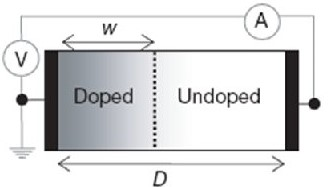
\includegraphics[width=\columnwidth]{memristor-w}
\caption{Left figure} \label{fig:left}
\end{subfigure}
\hfill
\begin{subfigure}{0.49\columnwidth}
\centering
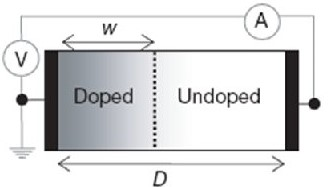
\includegraphics[width=\columnwidth]{memristor-w}
\caption{Right figure} \label{fig:right}
\end{subfigure}

\caption{}\label{}
\end{figure}

%% Lisajous Figures


\subsection{Modelo de Deriva Linear}

\section{Simulações} \label{sim}


\section{Aplicações}\label{aplicacoes}
\subsection{Mémorias ReRam}
A Memória Resistiva de Acesso Randômico (ReRAM), assim como a memória de acesso aleatório magnéticas (MRAM), mantêm os dados na falta de energia, essa propriedade deve-se especialmente pela presença do memristor em seus chips, que altera sua resistência à passagem da corrente elétrica em resposta a variações na sua tensão de alimentação.
Essa tecnologia assemelha ao uso de transistores nas memórias Flash, com a diferença de as células de memória ReRAM poderem ser muito menores, consumir menos energia elétrica e ter desempenho para leitura e escrita de dados próximos aos de módulos da Memória de Acesso Randômico Dinâmica (DRAM)\cite{blog} , que diferentemente da memória ReRAM (que armazena os dados como resistência), essa armazena os dados como carga elétrica.
O reRAM, portanto, tem o potencial de ser extremamente denso, de baixa potência, com alta resistência, tornando-se uma tecnologia atraente para armazenamento secundário e níveis de memória de classe de armazenamento \cite{prog}. Segundo a HP, dispositivos contendo memristores oferecem em média algo em torno de 20GB por centímetro quadrado, o dobro da capacidade projetada para as memórias flash \cite{hp}.
Dispositivos memresistivos podem mudar o paradigma padrão da computação ao permitir que cálculos sejam executados nos chips onde a informação está armazenada \cite{hp}. Além disso, essa tecnologia é passível de utilização em todo o tipo de dispositivo, desde celulares e MP3 players, que primariamente utilizam memórias flash NAND, como SSD (solid state disk, as memórias flash) e DRAM.

\subsection{Circuitos Lógicos} %  logic, hybrid circuits with CMOS, and neuromorphic computing.


\section{CONCLUSÕES}


%==================================
% REFERÊNCIAS
%==================================
\begin{thebibliography}{9}

%% INTRODUCAO
\bibitem{artigo}	
    L. Chua,
    “Memristor - the missing circuit element”, 
    in \emph{IEEE Transactions on circuit theory}, VOL. CT-18, NO. 5, Setembro 1971.

\bibitem{nature}	
     D.B. Strukov, G.S. Snider, D.R. Stewart,  R.S Williams, 
"The missing memristor found", 
\emph{Nature}, 2008, 1 May 2008, vol. 453, pp. 80-83.

\bibitem{memcomputacao}
    R. S. Pissardini,
    “MEMCOMPUTAÇÃO: CARACTERÍSTICAS E APLICAÇÕES EM
COMPUTAÇÃO PARALELA”, Escola Politécnica da Universidade de São Paulo, Departamento de Engenharia de Transportes, Laboratório de Topografia e Geodesia.
 Disponível em:
 \url{https://www.ime.usp.br/~gold/cursos/2015/MAC5742/reports/MemComputacao.pdf}. Acesso em: jun. 2019.
  


\begin{comment}
\bibitem{cibelly1}	
    D. Biolek, Z. Biolek, and V. Biolková, “\uppercase{SPICE modeling of memristive,
    memcapacitative and meminductive systems},” in Proc. of the European
    Conference on Circuit Theory and Design (ECCTD09), Antalya,
    Turkey, 2009, pp. 249-252. %% ainda não

\bibitem{cibelly2}	
    D. B. Strukov, G. S. Snider, D. R. Stewart, and R. S. Williams, “\uppercase{The
    missing memristor found}”, Nature, 2008, vol. 453, pp. 80–83. %% preciso baixar esse artigo
\end{comment}

%% FUNCIONAMENTO ESTRUTURAL
\bibitem{conceito}	
    J. P. Strachan, A. C. Torrezan, F. Miao, M. D. Pickett, J. J. Yang; W. Yi, G. M. Ribeiro, R. S. Williams, “STATE DYNAMICS AND MODELING OF TANTALUM OXIDE MEMRISTORS”, Disponível em: \url{https://ieeexplore.ieee.org/stamp/stamp.jsp?arnumber=6542012}. Acesso em ago. 2019.
    
\bibitem{us}	
    United States Patent; Patent No: US 9035272 B2. “NANOPARTICLE-BASED MEMRISTOR STRUCTURE”. Disponível em: \url{https://patentimages.storage.googleapis.com/0e/70/e0/6b8926f49e7cd8/US9035272.pdf}. Acesso em ago. 2019.
    
\bibitem{construcao}	
   F.S.Barachati, "ESTUDO E PREPARAÇÃO DE MEMORISTORES PARA SUA APLICAÇÃO EM DISPOSITIVOS ELETRÔNICOS". Escola de Engenharia de São Carlos, da Universidade de São Paulo. Disponível em: \url{http://www.tcc.sc.usp.br/tce/disponiveis/18/180450/tce-26032012-090929/publico/Barachati_Fabio_Souza.pdf}. 
   Acesso em ago. 2019.

%% MATEMATICA
\bibitem{elusive} % indescritivel
    Y. N. Joglekar, S. J. Wolf, "The elusive memristor: properties of basic electrical circuits", Department of Physics, Indiana University Purdue, 2009.

\bibitem{1976}	
    L. Chua, S. M. Kang,
    “Memristive devices and systems”, 
    in \emph{Proceedings IEEE}, 1976, vol. CT-18, no. 5, pp. 507-519.

%% APLICACOES

%% MEMORIAS RERAM
\bibitem{blog}
   E. Alecrim, "Os primeiros chips ReRAM fabricados em larga escala chegarão em breve", 2013. Disponível em: \url{https://tecnoblog.net/136874/primeiros-chips-reram-em-larga-escala/}. Acesso em ago. 2019.
   
\bibitem{prog}
    M. Ramadan, N. Wainstein, R. Ginosar, S. Kvatinsky, "Adaptive programming in multi-level cell ReRAM", Microelectronics Journal, Volume 90, 2019. %% MULTI-LEVEL CELL == MLC ?!
    %% bem recente :)
    
\bibitem{hp}
A. Martins, "ReRAM - A próxima geração de memórias e CPU’s", 2010. Disponível em: \url{https://brainstormdeti.wordpress.com/2010/09/15/reram-\%E2\%80\%93-a-proxima-geracao-de-memorias-e-cpu\%E2\%80\%99s/}. Acesso em ago.2019

%% CIRCUITOS LOGICOS


\end{thebibliography}



\end{multicols}
\end{document}
